%%%%%%%%%%%%%%%%%%%%%%%%%%%%%%%%%%%%%%%%%%%%%%%%%%%%%%%%%%%%%%%%%%%%%%%%%%%%%%%
% PREAMBOLO COMUNE PER APPUNTI (Stile Scuro)
%
% Questo file contiene tutte le impostazioni e i pacchetti comuni.
% NON contiene \begin{document} o \end{document}.
%
% Istruzioni per la compilazione del file principale:
% pdflatex -shell-escape nomefile_principale.tex
%%%%%%%%%%%%%%%%%%%%%%%%%%%%%%%%%%%%%%%%%%%%%%%%%%%%%%%%%%%%%%%%%%%%%%%%%%%%%%%

\documentclass{article}

% --- Encoding e lingua ---
\usepackage[utf8]{inputenc}
\usepackage[italian]{babel}

% --- Margini e layout ---
\usepackage{geometry}
\geometry{a4paper, margin=1in}

% --- Font sans-serif (come Helvetica) ---
\usepackage[scaled]{helvet}
\renewcommand{\familydefault}{\sfdefault}
\usepackage[T1]{fontenc}

% --- Matematica ---
\usepackage{amsmath}
\usepackage{amssymb}

% --- Liste personalizzate ---
\usepackage{enumitem}
% \setlist{nosep}

% --- Immagini e Grafica ---
\usepackage{float}
% \usepackage{graphicx}
\usepackage{tikz}
\usetikzlibrary{shapes.geometric, positioning, arrows.meta, calc, fit, backgrounds, patterns, decorations.pathreplacing}

% --- Tabelle Avanzate ---
\usepackage{array}
\usepackage{booktabs}
\usepackage{longtable}

% --- Hyperlink e Metadati PDF ---
\usepackage{hyperref}

\hypersetup{
    colorlinks=true,
    linkcolor=white,
    filecolor=magenta,
    urlcolor=cyan,
    citecolor=green,
    % pdftitle, pdfauthor, ecc. verranno impostati nel file principale
    pdfpagemode=FullScreen,
    bookmarksopen=true,
    bookmarksnumbered=true
}

% --- Licenza del documento ---
\usepackage[
  type={CC},
  modifier={by-sa},
  version={4.0},
]{doclicense}

% --- Colori e Sfondo Nero ---
\usepackage{xcolor}
\pagecolor{black}
\color{white}

% --- Evidenziazione del Codice ---
\usepackage{minted}
\setminted{
    frame=lines,
    framesep=2mm,
    fontsize=\small,
    breaklines=true,
    style=monokai,
    bgcolor=black!80
}
\usemintedstyle{monokai}

% --- Comandi personalizzati per algebra relazionale ---
\newcommand{\Rel}[1]{\textit{#1}} % Per i nomi delle relazioni
\newcommand{\Attr}[1]{\textsf{#1}} % Per i nomi degli attributi

\newcommand{\myunion}{\cup}
\newcommand{\myintersection}{\cap}
\newcommand{\mydifference}{-}
\newcommand{\myrename}[2]{\rho_{#1}(#2)}
\newcommand{\myselectop}[2]{\sigma_{#1}(#2)}
\newcommand{\myproject}[2]{\pi_{#1}(#2)}
\newcommand{\mycartesian}{\times}
\newcommand{\mynaturaljoin}{\bowtie} % Usare \Join da amssymb se disponibile e preferito
\newcommand{\mythetajoin}[3]{#1 \bowtie_{#2} #3} % R1 \bowtie_cond R2

% --- Comandi personalizzati per logica ---
\newcommand{\mylandop}{\wedge}
\newcommand{\myvel}{\vee}
\newcommand{\mynegop}{\neg}
\newcommand{\myforallop}{\forall}
\newcommand{\myexistsop}{\exists}

% --- Join esterni (outer join) ---
% Definizione standard per i join esterni
\def\ojoin{\setbox0=\hbox{$\mynaturaljoin$}%
	\rule[-.02ex]{.25em}{.4pt}\llap{\rule[\ht0]{.25em}{.4pt}}}
\newcommand{\myleftouterjoin}{\mathbin{\ojoin\mkern-5.8mu\mynaturaljoin}}
\newcommand{\myrightouterjoin}{\mathbin{\mynaturaljoin\mkern-5.8mu\ojoin}}
\newcommand{\myfullouterjoin}{\mathbin{\ojoin\mkern-5.8mu\mynaturaljoin\mkern-5.8mu\ojoin}}



% --- Titolo ---
\title{Livello Fisico e Segnali}
\author{Basato sulle slide del Prof. Luciano Bononi}
\date{\today}

\begin{document}

\maketitle
\tableofcontents
\newpage

\section{Background sul Livello Fisico (PHY) Wireless}
Il livello fisico (PHY) si occupa della trasmissione dei bit grezzi attraverso il canale di comunicazione wireless. Comprendere le sue basi è fondamentale per progettare e gestire reti wireless.

\subsection{Proprietà delle Onde Radio (RF - Radio Frequency)}

\subsubsection{Comprensione della Radio Frequenza}
\begin{itemize}
    \item \textbf{Generazione, Copertura e Propagazione:} Le onde RF sono energia elettromagnetica generata da corrente alternata (AC) ad alta frequenza che scorre in un'antenna. L'antenna converte la corrente elettrica ``cablata'' in onde RF e viceversa.
    \item \textbf{Pianificazione Wireless:} La comprensione di come le onde RF si generano e si propagano è cruciale per pianificare la copertura di una rete wireless e gestirla efficacemente.
\end{itemize}
\begin{center}
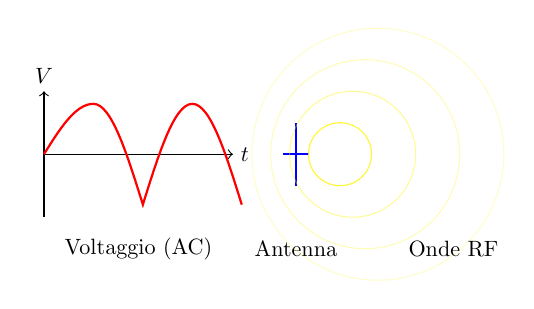
\begin{tikzpicture}[scale=0.8, every node/.style={transform shape}]
    % Voltaggio
    \draw[->] (0,0) -- (3,0) node[right] {$t$};
    \draw[->] (0,-1) -- (0,1) node[above] {$V$};
    \draw[red, thick] (0,0) sin (0.785,0.8) cos (1.57,-0.8) sin (2.355,0.8) cos (3.14,-0.8);
    \node at (1.5,-1.5) {Voltaggio (AC)};

    % Antenna
    \draw[thick, blue] (4,0.5) -- (4,-0.5); % Dipolo verticale
    \draw[thick, blue] (3.8,0) -- (4.2,0);   % Collegamento
    \node at (4,-1.5) {Antenna};

    % Onde RF
    \foreach \i in {1,2,3,4} {
        \draw[yellow, opacity=0.8/\i] (4.5+\i*0.2,0) circle (\i*0.5);
    }
    \node at (6.5,-1.5) {Onde RF};
\end{tikzpicture}
\end{center}

\subsubsection{Ampiezza (Amplitude)}
\begin{itemize}
    \item \textbf{Portata:} Segnali RF con ampiezza maggiore (più energia) tendono a propagarsi più lontano.
    \item \textbf{Potenza di Trasmissione (Watts):} È l'energia trasmessa per unità di tempo (Joule/Secondo).
    \[ \text{Potenza} = \text{Tensione} \times \text{Corrente} \]
    Maggiore tensione (energia) muove più elettroni (corrente).
\end{itemize}

\subsubsection{Frequenza (Frequency) e Lunghezza d'Onda (Wavelength)}
\begin{itemize}
    \item \textbf{Spettro Wireless:} L'insieme di tutte le possibili frequenze radio. Solo porzioni di questo spettro sono regolamentate e assegnate a specifiche tecnologie wireless.
    \item \textbf{Relazione:} $\lambda = \frac{c}{f}$
    dove $c$ è la velocità della luce (circa $3 \times 10^8 \, \text{m/s}$) e $f$ è la frequenza in Hertz (Hz).
    \item \textbf{Esempio Pratico (Banda ISM a \SI{2.4}{\giga\hertz}):}
    $f = \SI{2.4}{\giga\hertz} = 2.4 \times 10^9 \, \text{Hz}$
    \[ \lambda = \frac{3 \times 10^8 \, \text{m/s}}{2.4 \times 10^9 \, \text{Hz}} = 0.125 \, \text{m} = \SI{12.5}{\centi\meter} \]
    \item \textbf{Importanza Pratica per le Antenne:} Le antenne funzionano meglio quando la loro dimensione fisica è un multiplo o sottomultiplo della lunghezza d'onda (es. $1, \frac{1}{2}, \frac{1}{4}$ di $\lambda$).
\end{itemize}
\begin{center}
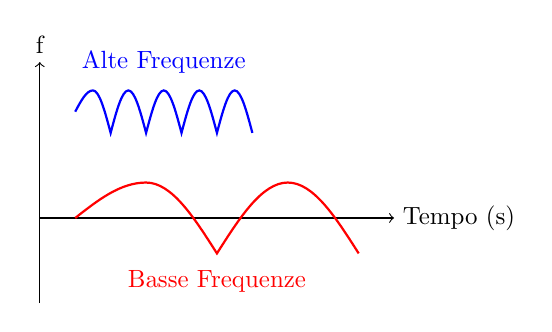
\begin{tikzpicture}[scale=0.9, every node/.style={transform shape}]
    \draw[->] (0,0) -- (5,0) node[right] {Tempo (s)};
    \draw[->] (0,-1.2) -- (0,2.2) node[above] {f};
    % Alta frequenza
    \draw[blue, thick] (0.5,1.5) sin (0.75,1.8) cos (1.0,1.2) sin (1.25,1.8) cos (1.5,1.2) sin (1.75,1.8) cos (2.0,1.2) sin (2.25,1.8) cos (2.5,1.2) sin (2.75,1.8) cos (3.0,1.2);
    \node[blue] at (1.75,2.2) {Alte Frequenze};
    % Bassa frequenza
    \draw[red, thick] (0.5,0) sin (1.5,0.5) cos (2.5,-0.5) sin (3.5,0.5) cos (4.5,-0.5);
    \node[red] at (2.5,-0.9) {Basse Frequenze};
\end{tikzpicture}
\end{center}

\subsubsection{Fase (Phase)}
\begin{itemize}
    \item \textbf{Definizione:} Sfasamento dell'onda rispetto a un punto di riferimento (gradi o radianti).
    \begin{itemize}
        \item Fase Positiva (left-shift): fronte d'onda anticipato.
        \item Fase Negativa (right-shift): fronte d'onda ritardato.
    \end{itemize}
    \item \textbf{Effetti Pratici (Eco e Interferenza):} Segnali riflessi (echi) arrivano con fasi diverse.
    \begin{itemize}
        \item Se \textbf{in fase}: interferenza costruttiva (segnale più forte).
        \item Se \textbf{in controfase} (sfasate di \SI{180}{\degree}): interferenza distruttiva (segnale più debole o nullo).
    \end{itemize}
\end{itemize}
\begin{center}
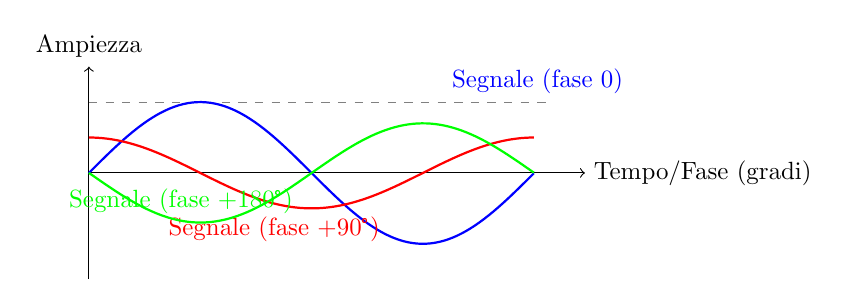
\begin{tikzpicture}[scale=0.9, every node/.style={transform shape}]
    \draw[->] (0,0) -- (7,0) node[right] {Tempo/Fase (gradi)};
    \draw[->] (0,-1.5) -- (0,1.5) node[above] {Ampiezza};
    % Segnale principale (fase 0)
    \draw[dashed, gray] (0,1) -- (6.5,1);
    \draw[thick, blue] plot[domain=0:6.28, samples=100] (\x, {sin(\x r)});
    \node[blue, above right] at (5,1) {Segnale (fase 0)};
    % Segnale sfasato +90
    \draw[thick, red] plot[domain=0:6.28, samples=100] (\x, {sin((\x+1.57) r)*0.5}); % 1.57 rad = 90 deg
    \node[red, below right] at (1,-0.5) {Segnale (fase +90°)};
    % Segnale sfasato +180
    \draw[thick, green] plot[domain=0:6.28, samples=100] (\x, {sin((\x+3.14) r)*0.7}); % 3.14 rad = 180 deg
    \node[green, above left] at (3,-0.7) {Segnale (fase +180°)};
\end{tikzpicture}
\end{center}

\subsubsection{Polarizzazione (Polarization)}
\begin{itemize}
    \item \textbf{Definizione:} Orientamento fisico dell'antenna, che determina l'orientamento del campo elettrico dell'onda RF.
    \item \textbf{Componenti Onda RF:} Campo Elettrico (E-field) e Campo Magnetico (H-field), perpendicolari tra loro.
    \item \textbf{Tipi Comuni:}
    \begin{itemize}
        \item Polarizzazione Orizzontale: Campo elettrico parallelo al suolo.
        \item Polarizzazione Verticale: Campo elettrico perpendicolare al suolo (comune nelle WLAN).
    \end{itemize}
    \item \textbf{Importanza Pratica:} Per comunicazione ottimale, le antenne trasmittente e ricevente dovrebbero avere la \textbf{stessa polarizzazione}. Disallineamenti causano perdita di segnale.
\end{itemize}
\begin{center}
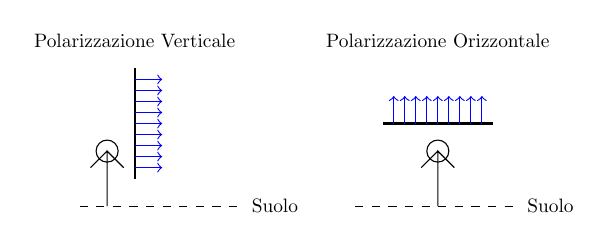
\begin{tikzpicture}[scale=0.7, every node/.style={transform shape}]
    % Polarizzazione Verticale
    \node at (-2, 2.5) {Polarizzazione Verticale};
    \draw[thick] (-2,0) -- (-2,2); % Antenna
    \foreach \i in {0.2,0.4,...,1.8} {
        \draw[blue, ->] (-2,\i) -- (-1.5,\i); % Campo Elettrico
    }
    \draw[dashed] (-3,-0.5) -- (0,-0.5) node[right] {Suolo};
    % Stickman
    \draw (-2.5, -0.5) -- (-2.5, 0.5) -- (-2.2, 0.2) -- (-2.5, 0.5) -- (-2.8, 0.2);
    \draw (-2.5,0.5) circle (0.2);


    % Polarizzazione Orizzontale
    \node at (3.5, 2.5) {Polarizzazione Orizzontale};
    \draw[thick] (2.5,1) -- (4.5,1); % Antenna
     \foreach \i in {2.7,2.9,...,4.3} {
        \draw[blue, ->] (\i,1) -- (\i,1.5); % Campo Elettrico (verso alto per visibilità)
    }
    \draw[dashed] (2,-0.5) -- (5,-0.5) node[right] {Suolo};
    % Stickman
    \draw (3.5, -0.5) -- (3.5, 0.5) -- (3.8, 0.2) -- (3.5, 0.5) -- (3.2, 0.2);
    \draw (3.5,0.5) circle (0.2);
\end{tikzpicture}
\end{center}
\textbf{N.B.:} Il problema della polarizzazione è molto importante per lunghe distanze e antenne direzionali. A breve distanza, le riflessioni mitigano il disallineamento.

\section{Propagazione RF e Comportamenti}

\subsection{Copertura della Trasmissione Radio}
\begin{itemize}
    \item \textbf{Attenuazione con la Distanza:} La potenza del segnale (P) diminuisce con $P \propto \frac{P_{tx}}{d^k}$.
    \begin{itemize}
        \item In spazio libero, $k \approx 2$.
        \item Con ostacoli, $k \ge 3$.
    \end{itemize}
    \item \textbf{Effetto della Potenza di Trasmissione ($P_{tx}$):} Aumentando $P_{tx}$, il segnale arriva più lontano.
\end{itemize}
\begin{center}
\begin{tikzpicture}[scale=0.9, every node/.style={transform shape}]
    % Sorgente
    \node[draw, circle, fill=blue!30] (A) at (0,0) {A};
    % Onde
    \draw[yellow, pattern=dots] (A) circle (2.5cm);
    \draw[yellow, opacity=0.5] (A) circle (2cm);
    \draw[yellow, opacity=0.8] (A) circle (1.5cm);
    % Grafico attenuazione
    \begin{scope}[xshift=5cm, yshift=-0.5cm]
        \draw[->] (0,0) -- (3.5,0) node[right] {$d$};
        \draw[->] (0,0) -- (0,2.5) node[above] {Potenza};
        \draw[red, thick] plot[smooth, domain=0.5:3] (\x, {2/\x});
        \node[red] at (1.5,2.2) {$\sim 4 P_{tx}$};
        \draw[yellow, thick] plot[smooth, domain=0.5:3] (\x, {0.5/\x});
        \node[yellow] at (2.5,0.8) {$P_{tx}$};
        \draw[cyan, dashed] (0,0.3) -- (3,0.3) node[right] {Limite rilevamento};
    \end{scope}
\end{tikzpicture}
\end{center}

\subsection{Portate (Ranges) della Propagazione del Segnale Wireless}
\begin{itemize}
    \item \textbf{Transmission Range:} Comunicazione possibile con basso tasso di errore.
    \item \textbf{Detection Range:} Segnale rilevabile, ma comunicazione non affidabile.
    \item \textbf{Interference Range:} Segnale abbastanza forte da interferire, anche se non rilevabile.
\end{itemize}
\textbf{Importante:} Queste portate \textbf{dipendono dalla sensibilità del ricevitore!}
\begin{center}
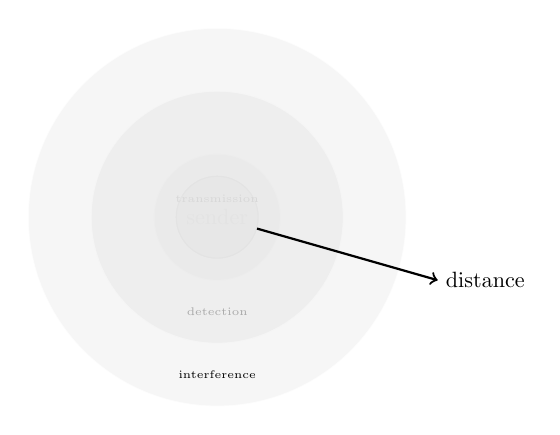
\begin{tikzpicture}[scale=0.8, every node/.style={transform shape}]
    \node[draw, circle, fill=gray!70] (sender) at (0,0) {sender};
    \draw[fill=gray!50, draw=white, opacity=0.7] (sender) circle (1cm);
    \node at (0,0.3cm) {\tiny transmission};
    \draw[fill=gray!30, draw=white, opacity=0.7] (sender) circle (2cm);
    \node at (0,-1.5cm) {\tiny detection};
    \draw[fill=gray!10, draw=white, opacity=0.7] (sender) circle (3cm);
    \node at (0,-2.5cm) {\tiny interference};
    \draw[->, thick] (sender) -- (3.5, -1) node[right] {distance};
\end{tikzpicture}
\end{center}

\subsection{Effetto degli Ostacoli}
Gli ostacoli possono \textbf{riflettere} o \textbf{assorbire} le onde RF. L'effetto dipende dal materiale e dalla frequenza.
\begin{itemize}
    \item \textbf{Alte Frequenze (es. \SI{5}{\giga\hertz}, \SI{6}{\giga\hertz}):} Più attenuate dagli ostacoli, migliori per brevi distanze.
    \item \textbf{Basse Frequenze (es. \SI{900}{\mega\hertz}):} Penetrano meglio gli ostacoli, migliori per lunghe distanze.
\end{itemize}

\subsection{Effetti della Propagazione del Segnale Wireless}
\begin{itemize}
    \item \textbf{Fading:} Fluttuazioni della potenza del segnale.
    \item \textbf{Shadowing:} Attenuazione da grossi ostacoli.
    \item \textbf{Reflection (Riflessione):} Rimbalzo su grandi superfici.
    \item \textbf{Refraction (Rifrazione):} Cambio direzione attraverso mezzi diversi.
    \item \textbf{Scattering (Diffusione):} Dispersione da piccoli ostacoli.
    \item \textbf{Diffraction (Diffrazione):} Piegamento attorno ai bordi.
\end{itemize}

\subsection{Propagazione Multipath (Percorsi Multipli)}
Il segnale raggiunge il ricevitore tramite percorsi multipli.
\begin{itemize}
    \item \textbf{Time Dispersion (Dispersione Temporale):} Copie del segnale arrivano in istanti diversi.
    \begin{itemize}
        \item \textbf{Inter-Symbol Interference (ISI):} Sovrapposizione di simboli, causa errori.
    \end{itemize}
    \item \textbf{Distorsione del Segnale:} Il segnale risultante è la somma di copie con fasi e ampiezze diverse.
\end{itemize}
\begin{center}
\begin{tikzpicture}[scale=0.8, every node/.style={transform shape}]
    \node (tx) at (0,1) [draw, trapezium, trapezium angle=60, minimum width=0.5cm, minimum height=1cm, fill=gray!30] {}; % Antenna TX
    \node (rx) at (6,1) [draw, trapezium, trapezium angle=60, minimum width=0.5cm, minimum height=1cm, fill=gray!30, shape border rotate=180] {}; % Antenna RX
    \node (building) at (3,2.5) [draw, fill=brown!50, minimum width=0.5cm, minimum height=1cm] {Edificio};
    \draw[->, thick, blue] (tx.east) -- (rx.west) node[midway, below, sloped] {LOS};
    \draw[->, thick, red] (tx.east) .. controls (1.5,2) and (2.5,2.8) .. (building.south) .. controls (3.5,2.8) and (4.5,2) .. (rx.west);
    \draw[->, thick, orange] (tx.east) .. controls (2,-0.5) and (4,-0.5) .. (rx.west);
    
    \node at (0,-1) {Segnale trasmesso:};
    \draw[thick] (1.5,-1) -- (1.5, -0.5); % singolo impulso

    \node at (4.5,-1) {Segnale ricevuto:};
    \draw[thick, blue] (5.8,-1) -- (5.8, -0.5); % LOS
    \draw[thick, red, opacity=0.7] (6.1,-1) -- (6.1, -0.7); % Riflesso 1
    \draw[thick, orange, opacity=0.5] (6.4,-1) -- (6.4, -0.6); % Riflesso 2
\end{tikzpicture}
\end{center}

\subsection{Effetti della Mobilità}
Il movimento cambia le caratteristiche del canale.
\begin{itemize}
    \item \textbf{Fading a Breve Termine (Short Term Fading):} Rapide fluttuazioni di potenza.
    \item \textbf{Fading a Lungo Termine (Long Term Fading):} Cambiamenti lenti nella potenza media.
\end{itemize}

\subsection{Voltage Standing Wave Ratio (VSWR)}
\begin{itemize}
    \item \textbf{Causa:} Discrepanza di impedenza (Ohm) tra trasmettitore, cavo, antenna.
    \item \textbf{Effetto (``Return Loss''):} Energia riflessa indietro verso il trasmettitore.
    \item \textbf{Misura:} Rapporto tra impedenze. Ideale 1:1.
    \item \textbf{Conseguenze Negative:} Danneggiamento Tx, instabilità.
    \item \textbf{Soluzione VSWR:} Usare componenti con la \textbf{stessa impedenza} (tipica \SI{50}{\ohm} nelle WLAN).
\end{itemize}
\begin{center}
\begin{tikzpicture}[scale=0.8, every node/.style={transform shape}]
    \node (tx) [draw, rectangle, fill=blue!30, minimum height=1cm, minimum width=1.5cm] at (0,0) {Trasmettitore $Z_{out}=\SI{75}{\ohm}$};
    \node (cable1) [draw, rectangle, fill=green!30, minimum height=0.5cm, minimum width=2cm] at (2.5,0) {Cavo $Z_c=\SI{75}{\ohm}$};
    \node (cable2) [draw, rectangle, fill=red!30, minimum height=0.5cm, minimum width=2cm] at (5.5,0) {Cavo $Z_c=\SI{50}{\ohm}$};
    \node (ant) [trapezium, draw, fill=yellow!30, minimum height=1cm, shape border rotate=270] at (7.5,0) {Antenna $Z_L=\SI{50}{\ohm}$};

    \draw (tx.east) -- (cable1.west);
    \node at (1.25,0.5) {VSWR 1:1};
    \draw (cable1.east) -- (cable2.west);
    \node at (4,0.5) {VSWR 1.5:1};
    \draw [dashed, red, <-] (4, -0.3) to [out=180,in=-45] (3.5,-0.8) node[below] {Riflessione};
    \draw (cable2.east) -- (ant.west);
    \node at (6.5,0.5) {VSWR 1:1};
\end{tikzpicture}
\end{center}

\section{Potenza e Misurazioni}

\subsection{Radiatore Intenzionale (IR) e EIRP}
\begin{itemize}
    \item \textbf{Radiatore Intenzionale (IR):} Dispositivo Tx RF + cavi + connettori (\textbf{esclusa} antenna).
    \item \textbf{Potenza di Uscita dell'IR:} Potenza all'uscita dell'ultimo connettore, prima dell'antenna.
    \item \textbf{Equivalent Isotropically Radiated Power (EIRP):} Potenza totale che irradierebbe un'antenna isotropica per produrre la stessa intensità di segnale nella direzione di massima emissione dell'antenna reale.
    \[ \text{EIRP} = \text{Potenza IR (all'antenna)} + \text{Guadagno Passivo Antenna} \]
    (Calcoli accurati si fanno in dB/dBm/dBi).
\end{itemize}

\subsection{Misurazione della Potenza}
\subsubsection{Watt (W) e milliwatt (mW)}
Unità di misura della potenza elettrica \textbf{assoluta}.
\begin{itemize}
    \item Potenza tipica RF per WLAN:
    \begin{itemize}
        \item Access Point (AP): \SIrange{30}{100}{\milli\watt} (fino a \SI{250}{\milli\watt} outdoor).
        \item Client: \SIrange{15}{30}{\milli\watt}.
    \end{itemize}
\end{itemize}

\subsubsection{Decibel (dB)}
Unità logaritmica per esprimere un \textbf{rapporto} tra due potenze (guadagno/perdita).
\[ \text{Guadagno/Perdita (dB)} = 10 \cdot \log_{10} \left( \frac{\text{Potenza}_{\text{uscita}}}{\text{Potenza}_{\text{ingresso}}} \right) \]
\begin{itemize}
    \item Valore dB positivo = guadagno; negativo = perdita.
    \item \textbf{Regole Pratiche Approssimate:}
    \begin{itemize}
        \item $\SI{-3}{dB} \approx 1/2 \text{ potenza}$
        \item $\SI{+3}{dB} \approx 2 \times \text{ potenza}$
        \item $\SI{-10}{dB} \approx 1/10 \text{ potenza}$
        \item $\SI{+10}{dB} \approx 10 \times \text{ potenza}$
    \end{itemize}
    \item \textbf{Vantaggio dei dB:} Guadagni e perdite si sommano algebricamente.
\end{itemize}

\subsubsection{dBm (Decibel-milliWatt)}
Unità logaritmica per misurare la potenza \textbf{assoluta}, con riferimento fisso a \SI{1}{\milli\watt}.
\[ \SI{0}{dBm} = \SI{1}{\milli\watt} \]
\[ \text{Potenza (dBm)} = 10 \cdot \log_{10} \left( \frac{\text{Potenza (mW)}}{\SI{1}{\milli\watt}} \right) \]
\begin{itemize}
    \item Esempi:
    \begin{itemize}
        \item \SI{100}{\milli\watt} = \SI{+20}{dBm}
        \item \SI{30}{\milli\watt} $\approx$ \SI{+14.77}{dBm}
    \end{itemize}
\end{itemize}
\begin{table}[H]
\centering
\caption{Tabella di Conversione mW -- dBm (approssimata)}
\begin{tabular}{|c|c|c|c|c|c|c|c|c|c|}
\hline
\textbf{dBm} & -30 & -20 & -10 & 0 & +3 & +10 & +20 & +30 & +40 \\ \hline
\textbf{Potenza} & \SI{1}{\micro\watt} & \SI{10}{\micro\watt} & \SI{0.1}{\milli\watt} & \SI{1}{\milli\watt} & \SI{2}{\milli\watt} & \SI{10}{\milli\watt} & \SI{100}{\milli\watt} & \SI{1}{\watt} & \SI{10}{\watt} \\ \hline
\end{tabular}
\label{tab:dbm_conversion}
\end{table}

\subsubsection{dBi (Decibel-isotropic)}
Guadagno passivo di un'antenna rispetto a un'antenna \textbf{isotropica} (ideale, 0 dBi gain). Le antenne reali concentrano energia, avendo dBi positivo nelle direzioni preferite.

\subsubsection{dBd (Decibel-dipole)}
Guadagno passivo di un'antenna rispetto a un'antenna \textbf{dipolo a mezz'onda}.
Un dipolo a mezz'onda ha circa $\SI{2.14}{dBi}$.
\[ \SI{0}{dBd} = \SI{2.14}{dBi} \]
\[ \text{Guadagno (dBi)} = \text{Guadagno (dBd)} + 2.14 \]

\subsection{Monitoraggio della Potenza (es. IEEE 802.11)}
\begin{itemize}
    \item \textbf{Necessità:} Per determinare soglia sensibilità, selezionare bitrate, verificare stato canale.
    \item \textbf{RSSI (Received Signal Strength Indicator):} Indice della potenza ricevuta.
    \item \textbf{Problema:} Scala RSSI \textbf{non standardizzata} tra produttori. Difficile confrontare dispositivi basandosi solo su RSSI grezzo. Meglio guardare al valore in dBm.
\end{itemize}

\section{Antenne}

\subsection{Questioni Generali}
\begin{itemize}
    \item \textbf{Funzione:} Convertono energia elettrica $\leftrightarrow$ onde RF.
    \item \textbf{Dimensione:} Correlata alla frequenza RF (lunghezza d'onda).
    \item \textbf{Forma:} Correlata al pattern di radiazione.
    \item \textbf{Posizionamento:} Cruciale per copertura e sicurezza.
\end{itemize}

\subsection{Antenna Omnidirezionale (es. Dipolo)}
Irradia potenza equamente attorno all'asse verticale (pattern a ``ciambella'').
\begin{itemize}
    \item \textbf{Dipolo a basso guadagno (es. \SI{2}{dBi}):} Ciambella più ``grassa'', buona copertura verticale.
    \item \textbf{Dipolo ad alto guadagno (es. \SIrange{8}{10}{dBi}):} Ciambella ``piatta'' e larga, buona copertura orizzontale estesa.
    \item \textbf{N.B.:} Segnale debole sopra/sotto un dipolo verticale (nel ``buco della ciambella'').
    \item \textbf{Tilt dell'Antenna (Inclinazione):} Inclinare un'antenna ad alto guadagno verso il basso (``downtilt'') migliora la copertura nell'area sottostante.
\end{itemize}
\begin{center}
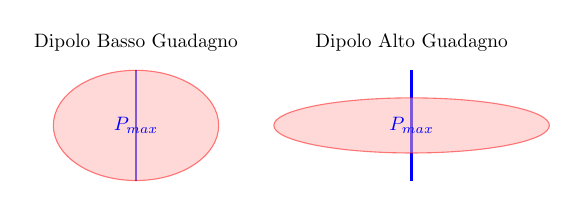
\begin{tikzpicture}[scale=0.7, every node/.style={transform shape}]
    % Low Gain Dipole
    \node at (0,2.5) {Dipolo Basso Guadagno};
    \draw[thick, blue] (0,0) -- (0,2); % antenna
    \draw[red, fill=red!30, opacity=0.5] (0,1) ellipse (1.5cm and 1cm); % pattern
    \node at (0,1) [blue] {$P_{max}$};

    % High Gain Dipole
    \node at (5,2.5) {Dipolo Alto Guadagno};
    \draw[thick, blue] (5,0) -- (5,2); % antenna
    \draw[red, fill=red!30, opacity=0.5] (5,1) ellipse (2.5cm and 0.5cm); % pattern
    \node at (5,1) [blue] {$P_{max}$};
\end{tikzpicture}
\end{center}

\subsection{Antenne Semi-Direzionali}
Concentrano energia in una direzione più specifica.
\begin{itemize}
    \item \textbf{Tipi:} Patch, Panel (piatte, a muro), Yagi (asta con ``baffi'').
    \item \textbf{Beamwidth (Larghezza del Fascio):} Angolo entro cui la potenza è almeno -3dB rispetto al massimo.
\end{itemize}

\subsection{Antenne Altamente-Direzionali}
Concentrano energia in un fascio molto stretto, alto guadagno.
\begin{itemize}
    \item \textbf{Tipi:} Parabolic Dish, Grid.
    \item \textbf{Uso Comune:} Link Punto-Punto (LOS).
    \item \textbf{Allineamento Critico.}
    \item \textbf{Fresnel Zone (Zona di Fresnel):} Spazio a forma di ellissoide attorno al LOS. La prima FZ deve essere il più libera possibile da ostruzioni.
    \begin{itemize}
        \item Raggio FZ dipende da distanza e frequenza, \textbf{non} dal tipo di antenna.
        \item Ostruzione < 20\% tollerabile.
        \item \textbf{Curvatura Terrestre:} Importante per link > \SI{10}{\kilo\meter}.
    \end{itemize}
\end{itemize}
\begin{center}
\begin{tikzpicture}[scale=0.8, every node/.style={transform shape}]
    \node (tx_ant) at (-3,0) [cylinder, draw, shape border rotate=90, aspect=0.3, minimum height=1cm, minimum width=0.5cm, fill=blue!30] {}; % Antenna TX
    \node (rx_ant) at (3,0) [cylinder, draw, shape border rotate=90, aspect=0.3, minimum height=1cm, minimum width=0.5cm, fill=blue!30] {}; % Antenna RX
    \draw[dashed, red] (tx_ant.east) -- (rx_ant.west) node [midway, above, font=\tiny] {LOS};
    % Fresnel Zone (1st)
    \draw[orange, fill=orange!30, opacity=0.5] (0,0) ellipse (3.2cm and 0.6cm);
    \node at (0,0) [font=\tiny, orange] {1a Zona Fresnel};
    % Obstacle
    \node (tree) at (0.5, -0.2) [circle, draw, minimum width=0.5cm, fill=green!50] {};
\end{tikzpicture}
\end{center}

\subsection{Antenne Settorizzate-Direzionali}
Array di antenne direzionali per coprire settori specifici. Permettono Space Multiplexing (riuso canali).

\subsection{Grafici di Copertura Antenna (Azimuth e Elevation)}
Diagrammi polari della potenza relativa nelle varie direzioni.
\begin{itemize}
    \item \textbf{Azimuth Chart:} Pattern visto dall'alto.
    \item \textbf{Elevation Chart:} Pattern visto di lato.
\end{itemize}

\subsection{Diversità delle Antenne (Antenna Diversity)}
Uso di più antenne per combattere il multipath fading.
\begin{itemize}
    \item \textbf{Switched/Selection Diversity:} Il ricevitore sceglie l'antenna con segnale migliore.
    \item \textbf{Diversity Combining:} I segnali vengono combinati (può richiedere cophasing).
\end{itemize}

\section{Path Loss e Link Budget}

\subsection{Path Loss (Perdita di Percorso)}
Attenuazione del segnale con distanza e frequenza.
\begin{itemize}
    \item Formula Free Space Path Loss (FSPL) (esempio):
    \[ \text{FSPL (dB)} = 32.4 + 20 \log_{10}(f_{\text{MHz}}) + 20 \log_{10}(d_{\text{km}}) \]
    \item \textbf{Regola dei 6 dB:} Ogni $\SI{+6}{dB}$ in EIRP (potenza x4) circa raddoppia la portata Tx (assumendo attenuazione $d^2$).
\end{itemize}
\begin{table}[H]
\centering
\caption{Esempio Path Loss 2.4 GHz vs Distanza (valori indicativi)}
\begin{tabular}{|c|c|c|}
\hline
\textbf{Distanza} & \textbf{Path Loss (dB)} & \textbf{Variazione approx.} \\ \hline
\SI{100}{\meter} & \SI{-80.2}{dB} & - \\ \hline
\SI{200}{\meter} & \SI{-86.2}{dB} & $\approx \SI{-6}{dB}$ \\ \hline
\SI{500}{\meter} & \SI{-94.2}{dB} & $\approx \SI{-8}{dB}$ \\ \hline
\SI{1000}{\meter} & \SI{-100.2}{dB} & $\approx \SI{-6}{dB}$ \\ \hline
\end{tabular}
\label{tab:path_loss}
\end{table}

\subsection{Calcolo del Link Budget (System Operating Margin)}
Eccesso di segnale rispetto al minimo necessario.
\begin{itemize}
    \item \textbf{Sensibilità del Ricevitore (RS):} Potenza minima (dBm) per decodifica affidabile. Più basso è, meglio è. Dipende dal bitrate.
    \item \textbf{Calcolo Potenza Ricevuta ($P_{RX}$):}
    \[ P_{RX} (\text{dBm}) = P_{TX} (\text{dBm}) + G_{TX} (\text{dBi}) + G_{RX} (\text{dBi}) - L_{\text{cavi}} (\text{dB}) - \text{PathLoss} (\text{dB}) \]
    \item \textbf{Link Budget (dB):}
    \[ \text{Link Budget} = P_{RX} (\text{dBm}) - RS (\text{dBm}) \]
    \item \textbf{Fade Margin (Margine di Fading):} Margine extra (tipico $\SIrange{+10}{+20}{dB}$) per fluttuazioni.
    \[ P_{RX} (\text{dBm}) > RS (\text{dBm}) + \text{Fade Margin (dB)} \]
\end{itemize}
\textbf{Esempio Link Budget (dalla slide 58, valori semplificati concettualmente):}
\begin{itemize}
    \item $P_{TX} = \SI{+15}{dBm}$
    \item $G_{TX} = \SI{+24}{dBi}$, $G_{RX} = \SI{+24}{dBi}$
    \item $L_{\text{cavi totali}} = \SI{10.8}{dB}$
    \item Path Loss (\SI{10}{km}) = $\SI{120}{dB}$
    \item $RS = \SI{-82}{dBm}$
    \item $P_{RX} = \SI{15}{dBm} + \SI{24}{dBi} + \SI{24}{dBi} - \SI{10.8}{dB} - \SI{120}{dB} = \SI{-67.8}{dBm}$
    \item Link Budget = $\SI{-67.8}{dBm} - (\SI{-82}{dBm}) = \SI{+14.2}{dB}$
\end{itemize}
Questo margine di $\SI{14.2}{dB}$ è disponibile per il fading. Se il fade margin richiesto è, ad esempio, $\SI{10}{dB}$, il link è considerato affidabile.

\end{document}